\subsubsection{GPS}
\chapterauthor{Johannes Treske}
Als GPS Modul haben wir das Modell GT-U7 von Goouuu Tech gewählt.
Dieses Modul kommuniziert über UART und sendet Nachrichten nach NMEA 0183 Standard.
In regelmäßigen Abständen sendet das GPS Modul die NMEA Sätze GGA, GLL, GSA, RMC, VTG und GSV.
Im Recommended Minimum Sentence C (RMC) sind fast alle für uns relevanten Informationen enthalten.
Dieser Satz gibt unter anderem Auskunft über das Datum und die Uhrzeit in UTC, sowie den Längen- und Breitengrad.
Der RMC Satz wird im Folgenden dargestellt:

\begin{center}
    \$GPRMC,HHMMSS,A,BBBB.BBBB,b,LLLLL.LLLL,l,GG.G,RR.R,DDMMYY,M.M,m,F*PP
\end{center}

Jeder NMEA Satz beginnt mit einem Dollarzeichen gefolgt von der Art des Satzes, im Beispiel RMC.
Alle weiteren Werte des Satzes werden durch ein Komma getrennt angegeben.
Ein Satz endet mit einem Asterisk gefolgt von zwei Byte Prüfsumme.
Diese Prüfsumme wird durch eine XOR Verknüpfung aller Nutzbytes berechnet.

Um das GPS Modul komfortabel nutzen zu können, werden Funktionen zum Auslesen von NMEA Sätzen, sowie zum Parsen der Sätze benötigt.

\begin{lstlisting}[language=C]
esp_err_t gpsReceiveNmea(char** nmea, size_t* len);
esp_err_t gpsParseNmea(char* nmea, size_t len, nmea_data_t* nmeaData, nmea_data_type_t* nmeaDataType);
\end{lstlisting}

Mit der \textit{gpsReceiveNmea} Funktion kann stets der nächste vollständige im Buffer gespeicherte NMEA ausgelesen werden.
Der Anfang eines Satzes wird durch das Dollarzeichen bestimmt, das Ende wird bei einem \glqq \textbackslash n\grqq\ erkannt.
Der aus dieser Funktion erhaltene Satz kann mit der Funktion \textit{gpsParseNmea} geparst werden.
Beim Parsen wird die Prüfsumme überprüft und falls diese korrekt ist, werden je nach Art des Satzes die einzelnen Werte des Satzes geparst.
Ist das Parsen erfolgreich, wird ein Objekt mit allen Werten, sowie die Art des NMEAs zurückgegeben.
Um einen bestimmten NMEA Satz zu erhalten, können diese beiden Funktionen in einer Schleife so lange aufgerufen werden, bis der gewünschte Satz gelesen wird.

\subsubsection{I2C-Sensoren}
\chapterauthor{Johannes Treske}
Im SunStorage Projekt werden neben dem GPS Sensor noch drei weitere Sensoren verwendet.
Der Beschleunigungssensor, der Temperatursensor und der Kompass werden über I2C angesprochen.
Das ESP-IDF Framework stellt bereits grundlegende Funktionen zur Kommunikation über I2C zur Verfügung.
Darauf aufbauend wurden Funktionen zum erleichterten Auslesen bzw. Schreiben von Registern der Sensoren geschrieben.
Diese können dann von den von uns geschriebenen Sensortreibern verwendet werden.
Die Treiber wurden hauptsächlich mithilfe der jeweiligen Datenblätter geschrieben.

\paragraph{Gyroskop/Beschleunigungssensor}
\chapterauthor{Johannes Treske}
Das Gyroskop bzw. der Beschleunigungssensor ist ein Modul, das mehrere Messwerte liefert.
Bei diesem Modul werden lediglich die Beschleunigungswerte verwendet, um die Schiefstellung des gesamten Systems zu ermitteln.
Der Treiber für dieses Modul umfasst Funktionen zum Initialisieren, Zurücksetzen, Schlafen legen, Auslesen der Messwerte und Einstellen der Messgenauigkeit.
Die Beschleunigungswerte werden auf drei Achsen gemessen und in G (also ungefähr $9.81\,\frac{m}{s^2}$) ausgegeben.

\paragraph{Barometer/Temperatursensor}
\chapterauthor{Johannes Treske}
Mit dem Barometer kann sowohl der Luftdruck als auch die Temperatur gemessen werden.
Im Projekt wird dieser Sensor verwendet, um die Temperatur der Batterie zu überwachen.
Der Treiber für diesen Sensor bietet die Möglichkeit Druck und Temperatur aus dem Sensor auszulesen, inklusive der Umrechnung der Rohdaten mithilfe der Kalibrierungsregister.
Die Kalibrierungsregister werden beim Initialisieren des Moduls ausgelesen und gespeichert.
Der Sensor gibt Druckwerte in Pascal und Temperaturwerte in Grad Celsius aus.

\paragraph{Kompass}
\chapterauthor{Johannes Treske und Felix Wagner}
Der Kompass bietet die Möglichkeit, die Ausrichtung des Systems zu berechnen.
Der Treiber für den Kompass gibt lediglich die Rohwerte der drei Achsen zurück.
Zur Berechnung der tatsächlichen Werte ist es notwendig, eine statische Kalibrierung vorzunehmen.
Eine Komponente der Kompassachse wird immer dann maximal, wenn die Achse nach Norden zeigt.\\

Die Kalibrierung wird wie folgt vorgenommen.
Die Sensoren, welche die Werte für die drei Achsen des Kompasses bestimmen, müssen zuerst auf ihre Maximal- und Minimalwerte überprüft werden.
Platziert man die ausgegebenen Werte der x- und y-Achse auf einem x-y-Koordinatensystem als Messpunkte, so bilden diese einen Kreis.
\begin{figure}[htpb] % {H}
    \centering
    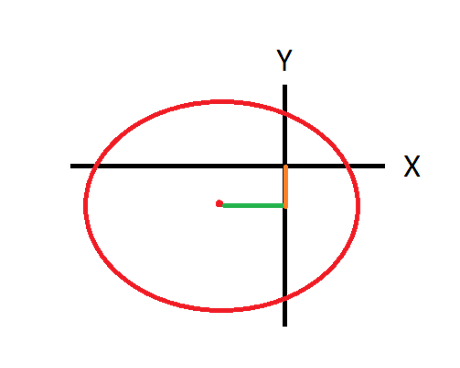
\includegraphics[scale=0.7,keepaspectratio=true]{pics/circle_offcenter.png}
    \caption{Kreis nicht im Ursprung}
    \label{fig:circle_offcenter}
\end{figure}
Um jeden Messpunkt zu erhalten, muss der Sensor einmal um alle Achsen gedreht werden.
Der entstehende Kreis ist ohne Kalibrierung nicht zentral im Koordinatensystem platziert.
Ziel ist es, den Kreis in den Koordinatenursprung zu verschieben.
\autoref{fig:circle_offcenter} zeigt nicht kalibrierten Zustand und \autoref{fig:circlecenter} den korrekt verschobenen Kreis.
\begin{figure}[htpb] % {H}
    \centering
    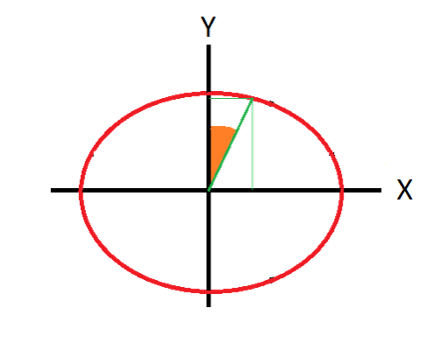
\includegraphics[scale=0.7,keepaspectratio=true]{pics/circle_center.png}
    \caption{Kreis im Ursprung}
    \label{fig:circlecenter}
\end{figure}

Für die Kalibrierung werden die Kompasswerte im Programmcode mehrmals pro Sekunde abgefragt und in Variablen gespeichert.
Dabei gibt es für jede Achse einen Minimal- und Maximalwert.
Nachdem der Kompass um alle drei Achsen gedreht wurde, sind die sechs Werte erfasst.
Anschließend muss daraus der jeweilige Korrekturfaktor für die einzelnen Achsen abgeleitet werden.
Ziel ist es, den Minimal- und Maximalwert für die Berechnung der Nordausrichtung im gleichen Abstand links und rechts des Koordinatenursprungs zu setzen, wie in \autoref{fig:circle_offcenter} gezeigt.
Dabei werden pro Achse die Maximalwerte und die Minimalwerte addiert und diese Summe halbiert.
Nun hat man die nötigen Korrekturfaktoren für die Kalibrierung und kann diese mit den x-, y- und z-Werte verrechnen.
Eine Eigenschaft des QMC5883L-Kompassmodul ist, dass dieses nicht ständig neu kalibriert werden muss.

\subsubsection{Servomotoren}
\chapterauthor{Felix Wagner}
Bei den Servomotoren handelt es sich um Analogservos der Firma Bluebird mit der Bezeichnung BMS-L530MG.
Diese benötigen eine Spannung von 4.5 V bis 6.5 V werden über ein PWM-Signal gesteuert.
Dieses Steuersignal hat eine Frequenz von 250 Hz und stellt den Servomotor bei einem Dutycycle von 1330 µs in seine mittlere Stellung.
Gegen den Uhrzeigersinn kann mit einem Dutycycle von 900 µs auf 60° gestellt werden.
Gleichfalls kann mit dem Dutycycle 2100 µs der Aktionsradius im Uhrzeigersinn gefahren werden.
Damit ergibt sich ein Gesamtaktionsbereich von 120°. \autocite{servomotor}

\paragraph{Ansteuerung}

\begin{figure}[htpb] % {H}
    \centering
    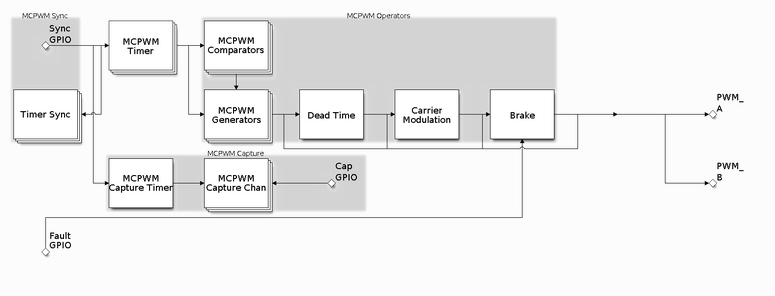
\includegraphics[scale=0.7,keepaspectratio=true]{pics/mcpwmOverview.png}
    \caption{MCPWM Überblick}
    \label{fig:mcpwmOverview}
\end{figure}

Die Generierung des PWM-Signals wird vom Neben-ESP übernommen.
Dafür wurde die MCPWM-Bibliothek verwendet.
\autocite{fig:mcpwmOverview} zeigt den Aufbau der Treiberbibliothek
Die folgenden Komponenten werden benötigt:

\begin{itemize}
    \item Timer: Zeitbasis des PWM-Signals
    \item Comparator: Vergleicht Zähler der Zeitbasis mit Schwellenwert und löst ein Vergleichsereignis aus
    \item Compare Event: Gibt das Verhalten vor, das bei einem positiven Vergleichen mit dem Dutycycle ausgeführt werden soll
    \item Generator: Generiert das PWM-Signal
    \item Operator: Modul, welches den Comparator und Generator zusammenführt, und somit die Signalerzeugung steuert
\end{itemize}

Der Timer wird mit einer Genauigkeit von 1 µs und einer Periode von 4000 eingestellt.
Dies entspricht 250 Hz.
Anschließend werden Comparator und Generator erstellt und mit dem Operator verknüpft.
Dann wird der Generator mit Verhaltensweisen konfiguriert, welche ausgeführt werden, wenn das Timerereignis und das Vergleichsereignis auftreten.
Tritt das Timerereignis auf, so wird das Signal am Portausgang auf \emph{HIGH} gesetzt.
Tritt nun das Vergleichsereignis auf, bei dem der Zeitzähler mit dem Wert des Dutycycles übereinstimmt, so wird der PWM-Port wieder auf \emph{LOW} gesetzt.
Der gewünschte Dutycycle wird durch die folgende Formel berechnet:

\[Dutycycle = angle_{required} \cdot \frac{PWM_{upper} - PWM_{lower}}{angle_{max}} + PWM_{lower} \]


\paragraph{Abdeckungsbereich}
Um die Solarpanele unabhängig der Sonnenposition ausrichten zu können, ist ein Gesamtaktionsbereich der Solarpanele von 360° Rotation nötig.
Jedoch besitzen die verbauten Servomotoren nur einen Aktionsradius von 120°. Da die Solarpanele so verbaut sind, dass sie sich in beide Richtungen gleich weit kippen lassen,
kann der Aktionsbereich verdoppelt werden.
Es verbleibt jeweils eine 60° breite Lücke auf beiden Seiten.\\
Umgesetzt wird dies wie Folgt:
Eine Funktion erhält die gewünschten Winkelpositionen für den Rotations- und den Kippservomotor und transformiert diese zunächst auf einen Wertebereich von 0° bis 360°.
Wird nun ein Winkel größer 180° für den Rotationsservo erkannt, so wird dieser Winkel um 180° verringert und zugleich vom Kippwinkel 180° abgezogen.
Damit kann fast die vollständige Abdeckung erreicht werden.

Anschließend wird der Berechnete Dutycycle vom maximalen höchsten Dutycycle abgezogen, um die Motoren mit steigendem Winkel gegen den Uhrzeigersinn drehen zu lassen.
Somit verhält sich der Ansteuerwinkel analog zu den Winkeln der Sonnenposition.

Um den Abdeckungsbereich der Servomotoren weiter zu erhöhen, wurde der minimale Dutycycle von 900 µs auf 820 µs verringert und der maximale Wert von 2100 µs auf 2150 µs erhöht.
Somit konnte der Abdeckungsbereich von 120° auf 160° erweitert werden.

\paragraph{Verbesserungen}
Die Servomotoren haben einige Probleme verursacht.
Die Anfangs gewählten Modelcraft ES-05 hatten durch ihre mangelhafte Dokumentation für großen Aufwand beim Suchen der korrekten Ansteuerung geführt.
Jedoch erwiesen sich diese Motoren für den Aufbau als zu schwach.
Somit musste auf die L530MG ausgewichen werden, welche jedoch nur einen Aktionsbereich von 120° gegenüber den 180° der ES-05 bieten. \\

Eine gute Alternative zu den Servomotoren wären Steppermotoren gewesen.
Diese hätten sich ebenfalls mit definierten Schritten mit ausreichender Genauigkeit positionieren lassen können.
Die günstigste Option hätte womöglich eine Kombination aus Linearmotor für die Rotation und Servomotor für die Kippfunktion geboten.
Hierbei würde das Kippen der Solarpanele analog zum aktuellen Aufbau funktionieren.
Die Rotation würde über den nicht positionierbaren Linearmotor müsste über einen, auf der Rotationsplattform platzierten, Kompasssensor überwacht werden.
Dabei muss zusätzlich auch auf mögliche Kabelverdrehungen geachtet werden, da beliebig weite Drehungen möglich sind.
